\problemname{Dalarna} 

\illustration{0.3}{dalarna.png}
\noindent
Harry älskar Dalarna och drömmer om att det ska bli Sveriges högst rankade län. 
Efter noggrann analys har han kommit fram till att om varje stad $i$ i Dalarna hade $p_i$ fler bilresor genom staden, 
skulle Dalarna ta förstaplatsen. För att uppnå detta planerar Harry att beställa taxibilar som kör mellan städerna, 
där varje bil ska färdas längs den kortaste vägen mellan två städer.

Dalarnas vägnät består av $N$ städer och $N-1$ vägar. Varje väg förbinder två städer direkt. Om en taxi befinner sig i en stad, 
kan den åka till alla städer som är direkt anslutna till den via en väg. Dessutom är nätverket konstruerat så att det alltid går att färdas mellan varje par av städer genom en eller flera vägar.

För varje stad $i$ behöver Harry se till att minst $p_i$ taxibilar passerar genom staden för att nå sitt mål. 
En taxibil åker mellan två bestämda städer i nätverket och färdas längs den kortaste vägen.

För att inte väcka misstankar vill Harry använda så få taxibilar som möjligt. 
Hjälp honom att räkna ut det minsta antal taxibilar han behöver beställa för att uppfylla kraven.


\section*{Indata}
Den första raden innehåller ett heltal $N$ ($1 \le N \le 10^5$), antalet städer i Dalarna.

Den andra raden innehåller $N$ heltal $p_1, p_2, ..., p_N$ ($0 \le p_i \le 10^9$), där $p_i$
anger hur många taxibilar som måste passera genom stad $i$.

De följande $N-1$ raderna beskriver vägarna mellan städerna. Varje rad innehåller två heltal $u$ och $v$
($1 \le u, v \le N$), vilket betyder att det finns en väg mellan stad $u$ och stad $v$.
Vägnätet sammankopplar alla städer.

\section*{Utdata}
Skriv ut ett heltal: det minsta antalet taxibilar som Harry behöver beställa.

\section*{Poängsättning}
Din lösning kommer att testas på en mängd testfallsgrupper.
För att få poäng för en grupp så måste du klara alla testfall i gruppen.

\noindent
\begin{tabular}{| l | l | p{12cm} |}
  \hline
  \textbf{Grupp} & \textbf{Poäng} & \textbf{Gränser} \\ \hline
  $1$    & $8$        & Det finns som mest $2$ vägar anslutna till vardera stad. \\ \hline
  $2$    & $11$       & $p_i = 1$ för alla $i$. \\ \hline
  $3$    & $9$        & $p_i \le 1$ för alla $i$. \\ \hline
  $4$    & $12$       & $N \le 7$, $p_i \le 5$ för alla $i$. \\ \hline
  $5$    & $14$       & $N \le 100$, $p_i \le 100$ för alla $i$. \\ \hline
  $6$    & $15$       & $N \le 1000$ \\ \hline
  $7$    & $31$       & Inga ytterligare begränsningar. \\ \hline
\end{tabular}


\begin{figure}[h!]
  \centering
  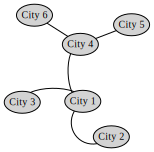
\includegraphics[width=0.3\textwidth]{dalarna_sample3.pdf}
  \caption{Vägnätverket för de 6 städerna i exempelfall 3.}
  \label{fig:dalarna_sample3}
\end{figure}

\begin{figure}[h!]
  \centering
  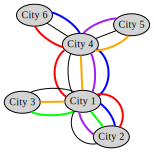
\includegraphics[width=0.3\textwidth]{dalarna_sample3b.pdf}
  \caption{En möjlig lösning för exempelfall 3, där de blåa, oranga, lila, gröna och röda vägarna är 5 olika taxibilars färd.}
  \label{fig:dalarna_sample3b}
\end{figure}